\documentclass[10pt,twocolumn,letterpaper]{article}

\usepackage{ijcb}
\usepackage{times}
\usepackage{epsfig}
\usepackage{graphicx}
\usepackage{amsmath}
\usepackage{amssymb}
\usepackage{mathtools}
\usepackage{cite}
\usepackage{algpseudocode}

\usepackage{url}
\urldef{\mailsa}\path|thomas.bergmueller@authenticvision.com| 
\urldef{\mailsb}\path|uhl@cosy.sbg.ac.at|
\newcommand{\keywords}[1]{\par\addvspace\baselineskip
\noindent\keywordname\enspace\ignorespaces#1}



\providecommand{\myceil}[1]{\left \lceil #1 \right \rceil }
\providecommand{\myfloor}[1]{\left \lfloor #1 \right \rfloor }


\providecommand{\etal}[0]{\textit{et al.} }


% Include other packages here, before hyperref.

% If you comment hyperref and then uncomment it, you should delete
% egpaper.aux before re-running latex.  (Or just hit 'q' on the first latex
% run, let it finish, and you should be clear).
%\usepackage[pagebackref=true,breaklinks=true,letterpaper=true,colorlinks,bookmarks=false]{hyperref}

%\ijcbfinalcopy % *** Uncomment this line for the final submission

\def\ijcbPaperID{****} % *** Enter the IJCB Paper ID here
\def\httilde{\mbox{\tt\raisebox{-.5ex}{\symbol{126}}}}

% Pages are numbered in submission mode, and unnumbered in camera-ready
\ifijcbfinal\pagestyle{empty}\fi
\begin{document}

%%%%%%%%% TITLE
\title{Impact of sensor ageing on iris recognition}

\author{Thomas Bergm{\"u}ller, Luca Debiasi and Andreas Uhl\\
University of Salzburg\\
Austria\\
{\tt\small \{ldebiasi,uhl\}@cosy.sbg.ac.at}
\and
Thomas Bergm{\"u}ller \\
Authentic Vision GmbH\\
Austria\\
{\tt\small thomas.bergmueller@authenticvision.com}
\and
Zhenan Sun\\
National Lab for Pattern Recognition CASIA\\
China\\
{\tt\small znsun@nlpr.ia.ac.cn}
}

\maketitle
\thispagestyle{empty}

%%%%%%%%% ABSTRACT
\begin{abstract}
   Similar to the impact of ageing on human beings, digital image sensors develop ageing effects over time. Since these imager's ageing effects (commonly denoted as pixel defects) leave marks in the captured images, it is not clear whether this affects the accuracy of iris recognition algorithms. This paper proposes a method to investigate the influence of sensor ageing on iris recognition by simulative ageing of an iris test database. A pixel model is introduced and an ageing algorithm is discussed to create the test database. To establish practical relevance, the simulation parameters are estimated from the observed ageing effects of a real iris scanner over the timespan of 4 years.
\end{abstract}

%%%%%%%%% BODY TEXT



\section{Introduction}
% TODO probably start with a quote
The ageing process starts immediately after being given birth. At first, ageing's aspects are considered to be rather positive. One grows up, gets stronger and learns new things. At a certain point, ageing starts to reveal several drawbacks. The skin gets wrinkled, joints and bones start to ache and our vision degenerates. In either case, ageing changes parts of our body. Although human beings change, others are still able to recognize people they knew before, even when they haven't met in a long time their appearance changed significantly.

Biometric systems aim to identify human beings by analysing their biometric samples, i.e. face, fingerprints or iris \cite{rathgeb}. These systems operate in two steps. In the enrollment process, a subject's biometric samples are registered for the first time and stored in a database. Later, in the authentication procedure, another sample is taken and compared to the one stored in the database to verify a subject's identity. Since there may be years or decades between enrollment and authentication, one strives to use biometric samples which are stable over time. The iris has been assumed to be stable, although it is currently topic of intensive discussion if and which iris-related information eventually changes as a human being ages. Some researchers claim that iris-related information is stable or relatively stable \cite{daugmanNoChange,BGrother13a}, while others observe significant changes over time \cite{rankinChange, rankinChangeResponse, fenkerIrisAging, czajkaTemplateAging, fairhurstNonstability}. Researchers mostly conclude these age-dependent changes in iris texture by observing changes in a system's iris-recognition rate. It is not clear, if observed changes in an algorithms' behaviour are caused by the ageing of the tested subject, which is commonly assumed, ageing of the recognition system itself or if this is caused by other unspecified factors.

This paper proposes a method to investitage the ageing impact of digital image sensors, which are crucial components of iris recognition systems. As a human being's vision often gets weaker with age, pixels start to get defective in image sensors over the years as well. This influences the quality - and therefore the appearance - of the captured images. Similar to being able to estimate a human being's age by their appearance, pixel defects observed in the captured images can reveal the age of the corresponding imager. This is used in image forensics to approximate the capturing date of an image \cite{fridrich}. Since the ageing effects of the sensor can be traced by evaluation of its output, namely the images, this implies that the capturing process is not time invariant. Hence two images, which capture the same (unchanged) scene, but were taken at significantly different points in time, may differ due to meanwhile developed sensor defects.

Digital image sensors are used to capture the iris features in the enrollment and the authentication process. It is not clear yet, whether the ageing of the sensor - and thus the development of ageing effects between taking two samples - influences the accuracy of iris recognition algorithms. To investigate this issue, one would need to have identical data captured at at least two significantly different points in time. It is practically impossible to establish identical conditions for both acquisitions. Furthermore, as mentioned, it is not possible to distinguish between the influence of the subject's and the sensor's ageing on iris recognition algorithms. For this reason one cannot capture test data to investigate the sensor's or the subject's ageing in an isolated manner physically. There is no way to explicitely examine the iris texture's ageing at all. However, it is possible to investigate the sensor ageing's influence on the iris recognition rate independent from the subject's ageing.

We propose a method to investigate the impact of sensor ageing on the iris recognition accuracy. This is done by generating simulatively aged test data, which contains sensor ageing related defects
%, based on an uncompressed iris database
(see section \ref{virtualAging}). The practical relevance of the simulation is ensured by estimating parameters from an iris database (section \ref{hotPixelRate}), where the same subjects were captured by the same sensor in 2009 and 2013 (section \ref{testing}). This test data set is used to test six implementations of iris recognition algorithms available in the University of Salzburg Iris Toolkit USIT (http://www.wavelab.at/sources). By observing changes in the EER for certain algorithms, we conclude on the impact of sensor ageing on iris recognition systems in section \ref{conclusion}.


\section{Sensor Aging and Pixel Model}
\label{sec:ageingAndPixelModel}
An image sensor is a two dimensional array of photosensitive cells called pixels. The purpose of an image sensor is to convert the incoming light to its digital representation, commonly denoted as the image \cite{imageSensors}. In theory, each pixel has the same rectangular shape and a unified photo-response, meaning all pixels should produce the same output value on unified incoming light. Due to imperfections in the manufacturing process, this is not the case in practice, hence there are pixels which are more sensitive than others \cite{camAndDisplays}. Besides that, some of a sensor's pixels might change their initial photo-response characteristics over a sensor's lifetime. We denote this defect-development over time as \emph{sensor ageing}.


\begin{figure}
\centering
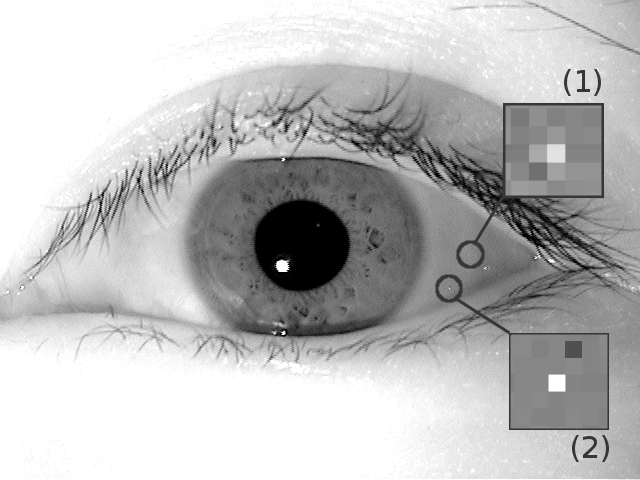
\includegraphics[width=0.7\linewidth]{img/defects.png}
%\caption{A \emph{partially-stuck or hot pixel} (1) and two \emph{stuck pixels} (2) in an iris image. Contrast has been enhanced in the close-ups for visualisation. Note that the partially-stuck pixel still corresponds to the incoming light, but is significantly brighter compared to its neighbours, while the stuck pixel are light-independent and yield to a constant output.  }
\caption{A \emph{partially-stuck or hot pixel} (1) and two \emph{stuck pixels} (2) in an iris image. Contrast has been enhanced in the close-ups for visualisation.}
\label{fig:hotStuck}
\end{figure}

The most common defects occuring over time are partially and fully stuck pixels, illustrated in fig. \ref{fig:hotStuck}. The photo-response of partially-stuck pixels tends to have a moderate offset, but still responds to the incident light. Stuck pixels produce a completely light-independent output value \cite{fridrich}. As soon as a pixel is defective, it remains defective over the rest of the sensor's lifetime \cite{failureSemi}. So one can obtain the important property that if a pixel is \emph{once defective, it remains defective}.

Related work \cite{datingImages, inFieldDefects, defectDetection,failureSemi, defectIdentification, fridrich} shows that the occurrence of new pixel defects is increasing linear with time. Defect locations are uniformly distributed and independent. Already known defects remain constant in respect to their location and type . 
To run a simulation, a model for calculating the pixel values of an image $Y$ has to be defined. There exist several pixel output models, which consider the incoming light and the impact of pixel defects on the raw output of a sensor. We denote $w,h \in \mathbb{Z}$ as the rows and columns of the sensor and start by adopting the model proposed in \cite{fridrich}:

\begin{equation}
\begin{aligned}
 Y = I+I \circ K+\tau D +c+\Theta \\ with \quad Y,I,K,D,C, \Theta \in \mathbb{R}^{w \times h}; \tau \in \mathbb{R}
\end{aligned}
  \label{equ:pixelmodel}
 \end{equation}

where the matrix $Y$ is the sensor output, commonly denoted as image, $I$ the intensity of incoming light, $I \circ K$ the photo-response non-uniformity PRNU, $\tau D$ the dark current (with $\tau$ being a multiplicative-factor representing exposure settings, sensor temperature, \dots), $C$ a light-independent offset and $\Theta$ some modeling noise. Since all pixels are independent \cite{fridrich, defectDetection} and all operations element-wise, we denote the matrix-elements $y_{x,y} \in Y$ as $ y \in Y$ for simplicity reasons. The same applies to $i \in I$, $k \in K$, $d \in D$, $c \in C$ and $\theta \in \Theta$.

Since we are interested in simulation of the ageing effects of a specific sensor, all age-independent defects, which are e.g. due to production process, can be eliminated. Hence the PRNU, which corresponds to the non-uniformity of pixel-dimensions, can be omitted. As we aim for reproducable tests, environmental influence (e.g. temperature) and modelling noise should be minimized. They can be eliminated completely in a simulation, thus we set $k=\theta=0$. Also the same exposure settings have to be used for the sensor in every test, therefore we have $\tau = const$ and set $ \tau = 1$ for simplicity. \cite{camAndDisplays, radiometricCCD,failureSemi,fridrich} suggest that the dark current is very weak with short exposure, which is necessary for applications in biometric systems to avoid motion blur. Under these considerations, a fairly simple model for a pixel's output which considers only ageing-relevant defects remains:

\begin{equation}
  \label{equ:pixemodelEasier}
  y = i + d + c \quad with \quad y,i,c \in \mathbb{R}
\end{equation}

Common defect types that develop over time as the sensor ages are stuck and hot pixels, where the definitions are quite contrary in literature (e.g. in \cite{fridrich, defectIdentification, failureSemi}). If the dark current $d$ of a pixel is extremely high, this is often denoted as a hot pixel. If the offset $c$ is high, this results in a saturated pixel and is called a stuck pixel according to \cite{fridrich}. \cite{defectIdentification}, however, suggests that a stuck pixel is not necessarily saturated but can obtain any value within the sensor output's universe. For the reason of non-uniform definitions we define the following models for defective pixels:

\begin{eqnarray}
  y & = & c \label{equ:Stuck} \\
  y & = & i + d \label{equ:Hot}
\end{eqnarray}
  
where the defect type in equ. (\ref{equ:Stuck}) is light-independent (thus referred as a \emph{stuck pixel}) and the one in equ. (\ref{equ:Hot}) adds an offset to the incident light and is commonly referred as either a partially-stuck or hot pixel. The dark current (which is the cause for hot pixels) depends on exposure time and temperature, which are both kept constant in this experiment. Thus also the dark current is constant and therefore there is no difference between a hot and a partially stuck pixel for this setup - therefore we denote this defect as a \emph{partially-stuck pixel}. In conclusion (and considering 8 bit grayscale images), the following pixel output model is definied:

\begin{equation}
\begin{aligned}
Y({x,y}) = \begin{cases}
C({x,y})  & \text{if $C({x,y}) \neq 0$}; \\
I({x,y}) +D({x,y})  & \text{otherwise}.\\
\end{cases} \\ \text{with} \quad Y,C,I,D \in {(\mathbb{Z}:[0;255])}^{w \times h}
\label{equ:finalPixelModel}
\end{aligned} 
\end{equation}

where a pixel's output $Y({x,y})$ saturates at $0$ and $255$ if interval borders are exceeded.

\section{Simulated sensor ageing}
\label{virtualAging}
For an ideal sensor, the defect matrices $C$ and $D$ are time-invariant zero matrices. As discussed, for real sensors pixel defects start to occur from a specific point in time $T_0$ with a constant rate. This can be modelled by a poisson process \cite{fridrich}. Therefore the number of stuck and partially-stuck pixels, denoted as $n_{s}$ and $n_{ps}$ respectively, at time $T$ are calculated as

\begin{eqnarray}
   n_s(T)  & = & (T-T_0) \lambda_s \\
  n_{ps}(T) & = &  (T-T_0) \lambda_{ps}
\end{eqnarray}

where $\lambda_s$ and $\lambda_{ps}$ are the growth rates, at which the particular defect types occur. Due to defects being independent of each other, the locations of defects in a 2D sensor array can be modelled by uniform distribution. Hence the position  $s_k \in {w \times h}$ of $k$-th defect is obtained from uniformly distributed random variables in the simulation. Depending on the $k$-th defect being a stuck or partially stuck pixel, the values of $C$ and $D$ (see equ. (\ref{equ:finalPixelModel})) have to be set. We denote $a_s$ as the maximum amplitude of a stuck pixel and $a_{ps}$ the maximum amplitude of a partially stuck pixel. Let $r_a \in \mathbb{R}:[0;1]$ be a uniformly distributed random number. Then we either have

\begin{eqnarray}
   C({s_k})  & = & r_a  a_s \quad \text{for a stuck pixel at } s_k \text{ or} \label{equ:stucks} \\
   D({s_k}) & = &  r_a a_{ps} \quad \text{for a partially-stuck pixel at } s_k \label{equ:partiallyStuck}
\end{eqnarray}


\subsection{Generation of virtually aged data}
These definitions are used, according to the pixel model in equ. (\ref{equ:finalPixelModel}), to add ageing-related sensor defects to an existing image $Y_{T_0}$, which was captured at ${T_0}$. One might argue that $Y_{T_0}$ already contains pixel defects since the some of the used sensor's pixels might be defective at $T_0$ already. Since we are only interested in investigating changes over a period of time, it does not matter which time frame is observed. This means, already contained defects in $Y_{T_0}$ do not influence the outcome of the experiment because we get relative results only. Sensor defects corresponding to a sensor's physical condition at a specific time $T_i$ are added to the image $Y_{T_0}$. The resulting image $Y_{T_i}$, subsequently denoted as \emph{aged image}, captures the same scene as in $T_0$, but suffers from the impact of ageing defects occured over time ${T_i} - {T_0}$. To investigate the behaviour of iris recognition algorithms, we compute a sequence of aged images $(Y_{T_i})_{i=1 \dots m}$. To do so, first a series of defect matrices, which represent the state of ageing at a specific point in time $T_i$, is calculated. We denote these sequences for sample points $T_0$ \dots $T_m$ as

\begin{equation}
(D_{T_i})_{i=0..m} \text{ and } (C_{T_i})_{i=0..m}
\end{equation}

The following algorithm is proposed to compute the sequence defect matrices and the sequence of aged images $Y_{T_i}$. Based on a source image $Y_{T_0}$ we have for sample points $T_0$ \dots $T_m$:

\vspace{2mm}
\begin{algorithmic}[1]

\Procedure{AgedImageSequence}{$Y_{T_0}$}

\For{$i=1 \dots m$}
\State $\Delta n_s\gets n_s(T_i - T_0) - n_s(T_{i-1} - T_0) $ 
\State $\Delta n_{ps}\gets n_{ps}(T_i - T_0) - n_{ps}(T_{i-1} - T_0) $
\State $D_{T_i}$ = $D_{T_{i-1}}$
\State $C_{T_i}$ = $C_{T_{i-1}}$

  \For{$k=1 \dots \Delta n_s$}
    \State $r_a \gets$ random in $[0;1]$
    \State $s_k \gets$ random in $w \times h$
    \State $C_{T_{i}}(s_k) \gets r_a \cdot a_s$ (equ. \ref{equ:stucks})
  \EndFor
  
  \For{$k=1 \dots \Delta n_{ps}$}
    \State $r_a \gets$ random in $[0;1]$ 
    \State $s_k \gets$ random in $w \times h$
    \State $D_{T_i}({s_k}) \gets r_a \cdot a_{ps}$ (equ. \ref{equ:partiallyStuck})
  \EndFor
  
  
  $Y_{T_{i}}(x,y) = \begin{cases}
  C_{T_i}(x,y) \quad \text{if $C_{T_i}(x,y) \neq 0$}; \\
  Y_{T_{0}}(x,y) +D_{T_i}(x,y)  \quad \text{otherwise}.
  \end{cases}$
  
\EndFor
\State \textbf{return} $(Y_{T_i})_{i=1 \dots m}$
\EndProcedure
\end{algorithmic}

\vspace{5mm}


The defect matrices $D$ and $C$ are computed recursively to satisfy the \emph{once defective, always defective} condition, hence arlier developed defects are maintained over virtual age. For each step, the numbers of defects $\Delta n_s$ and $\Delta n_{ps}$, which has to be added to the ones in the previous step, are calculated. Location and amplitude for the defects in the $i$-th ageing step are computed using random numbers. The defect matrices $C_{T_i}$ and $D_{T_i}$ are used to compute an aged image $Y_{T_i}$. Instead of the incident light $I$, the base image $Y_{T_0}$ can be used due to the given arguments of relative evaluation. This algorithm outputs a sequence of aged images $(Y_{T_i})_{i=1 \dots m}$. Each pixel $y_{T_i}$ in this sequence stores the incident light as in $Y_{T_0}$. Additionally it carries information related to the developed age-dependent defects in the time span $T_i-T_0$.
 
 
 
 
 \subsection{Parameter estimation from iris databases}
 \label{hotPixelRate}
 For the discussed simulative ageing process, the defect growth rates and amplitudes have to be defined. In laboratory set-ups, hot and \emph{partially stuck pixels} are usually identified by dark calibration tests (i.e. $I=0$) \cite{defectIdentification}. To the best of the authors' knowledge, there is no suitable laboratory-captured data set available for iris imagers. There are databases \cite{czajkaTemplateAging,fenkerIrisAging} available, which were acquired using the same equipment at two significantly different dates for the purpose of investigating iris texture ageing. In the following we propose a method to estimate the growth rates and amplitudes of stuck and partially-stuck  pixels from such databases. 
 
For the pixel model in equ. (\ref{equ:finalPixelModel}), the growth rates and amplitudes of stuck and partially-stuck pixels have to be detected. As discussed, these defects are usually detected from a single image when the incident light I is uniform and known, i.e. $I=0$. Hence only the defects $\Xi = D+C = Y-I$ remain. Because $I$ is random and non-uniform in our database, a statistical approach has to be used.
We denote a sequence of $K$ images taken in a very short period of time $Y_0 \dots Y_K$. 
%A partially-stuck pixel at position $(x,y)$ adds an light-independent offset to each pixel output $y_k = Y_k({x,y})$ on this position (refer equ. (\ref{equ:finalPixelModel})). 
A \emph{stuck pixel} obtains the same value in each image in this sequence (refer equ. (\ref{equ:finalPixelModel})). Hence a pixel at position $(x,y)$ is identified as being stuck iff

\begin{equation}
y_{0} = y_{1} = \dots = y_{K} \label{equ:conditionStuck}
\end{equation}

A partially-stuck pixel at position $(x,y)$ adds an light-independent offset to each pixel output $y_k = Y_k({x,y})$ on this position. We compute a pixel's mean $\bar{y}$ from the sequence of images and substitute the pixel values by the model in equ. (\ref{equ:finalPixelModel}). Because the possibility of a specific pixel being stuck can be ruled out by equ. (\ref{equ:conditionStuck}), $c$ is not considered here. In equ. (\ref{equ:modelWithNoise}) some modelling noise $\theta$ is added to cover impredicatable and diverse impacts in acquisition.
\begin{eqnarray}
\bar{y} & = & \frac{1}{K}\sum\limits_{k=1}^{K}y_k \\
\bar{y} & = & \frac{1}{K}\sum\limits_{k=1}^{K}(i_k+d+\theta_k) \label{equ:modelWithNoise}
\end{eqnarray}
The mean of a uniformly distributed modelling noise $\theta$ cancels out for sufficiently large $K$. We assume there are no pixel defects present, hence the offset $(d=0) \rightarrow d'$. Under this assumption we can substitute $i_k = y_k$ and denote the pixel mean $\bar{y}$ as $\bar{y}'$. The partially-stuck defect matrix $d$, although set to zero, contributes to each pixel output uniformly, thus it is independent of $k$, as shown in equ. (\ref{equ:modelWithD}). Under the assumption of no pixel defects, the identity $\bar{y}' \equiv median(y,q)$ holds, if the pixel means $\bar{y}$ have mostly identical values in a local $q \times q$ neighbourhood. This is the case in dark calibration tests, but also when only pixel mean of image regions are considered, where mostly unified brightness and texture are present, i.e. regions showing skin. This is why other regions, e.g. the regions where the iris usually is, have to be masked out, as illustrated in fig. \ref{fig:correlated}. 

\begin{figure}[h]
  \centering
  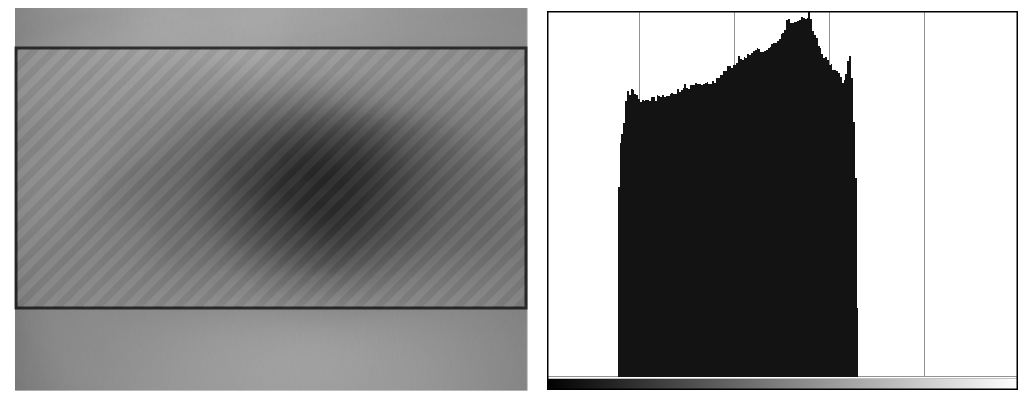
\includegraphics[width=\linewidth]{img/correlated.png}
  \caption{The mean image of $Y_1 \dots Y_k$ (left) has correlated data in the image's centre because of the iris usually being there. This (marked) region is not considered when detecting sensor defects. The histogram (right) of the uncorrelated top and bottom regions is indeed similar to uniform distribution.}
  \label{fig:correlated}
\end{figure}

By the non-linear nature of median, sparse outliers within the $q \times q$ neighbourhood are filtered  \cite{fridrich}. Such outliers occur, if - contrary to the assumption - there is a pixel defect. Hence with the median we have a method to compute the pixel mean $\bar{y}'$ disregarding the influence of pixel defects. We use this relation in equ. (\ref{equ:d}) to set $\bar{y}' \rightarrow median(y,q)$ and have $d' \rightarrow \hat{d}$ being an estimator for the offset, which is added to the incident light $i_k$ in a sensors pixel output $y_k$.
\begin{eqnarray}
\bar{y}' & = & d'+\frac{1}{K}\sum\limits_{k=1}^{K}(y_k) \label{equ:modelWithD} \\
\hat{d} & = & \frac{1}{K}\sum\limits_{k=1}^{K}y_k - median(\bar{y},q) \label{equ:d}
\end{eqnarray}

Amongst the partially-stuck pixel information, also information about the PRNU is also contained in $\hat{d}$. Since PRNU is caused by imperfections in the manufacturing process, it is likely to be normally distributed, which reflects in the logarithmic histogram of $\hat{d}$ in fig. \ref{fig:defectMat}. Therefore the median kernel size $q$ has to be chosen large enough to minimize the influence of PRNU on the median $med(\bar{y},q)$, which is the case if a normal distribution within the $q \ times q$-neighbourhood is observed as well.

\begin{figure}
  \centering
  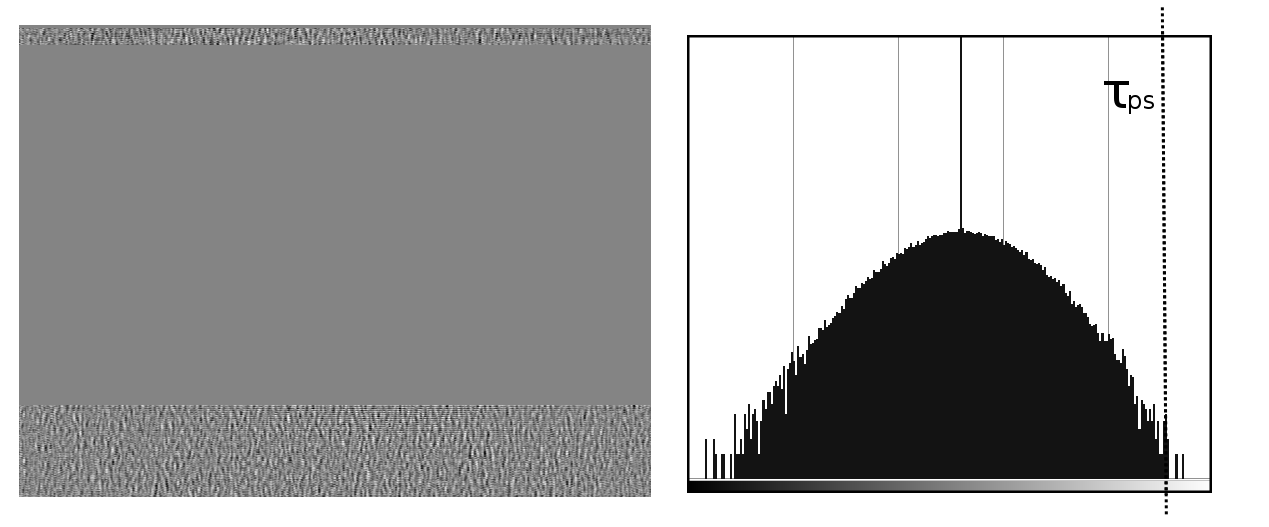
\includegraphics[width=\linewidth]{img/defectMatWithTau.png}
  \caption{The estimated offset matrix $\hat{D}$ (left, enhanced for visualisation) is calculated by equ. (\ref{equ:d}). The logarithmic histogram (right) of the uncorrelated regions shows a normal distribution, which is due to PRNU. The decision threshold $\tau_{ps}$ is chosen in a way that only outliers are declared as partially stuck pixels}
  \label{fig:defectMat}
\end{figure}


We declare a pixel to be partially stuck if $\hat{d}$ is an outlier in respect to the normal distribution and therefore has much higher sensivitiy than expected from PRNU. This is decided by checking for a certain threshold $\hat{d} > \tau_{ps}$. The decision threshold is chosen manually. We exploit the \emph{once defective, always defective}-property to guarantee a correct growth rate, even if $\tau_{ps}$ has been slightly off and therefore there was misclassification. We know that a sensor's partially-stuck pixels from $T_1$ also have to be present in $T_2$, which is illustrated in fig. \ref{fig:defectPersistence}. The number of defects $n_{match}$, which are present at the same location $s_k$ in the images captured at $T_1$ and $T_2$ can be determined. Considering the number of defects $n_1$ in the image captured at $T_1$, the correction factor $\gamma$ of the algorithm can be calculated as
\begin{equation}
\gamma = \frac{n_{match}}{n_1}
\end{equation}

Assuming that for $T_1$ and $T_2$ the same error is made, the observed increase of defects can be corrected with $\gamma$. Taking into account the size of the sensor $w\cdot h$, we retrieve the simulation parameters by the following relations: 

\begin{figure}
  \centering
  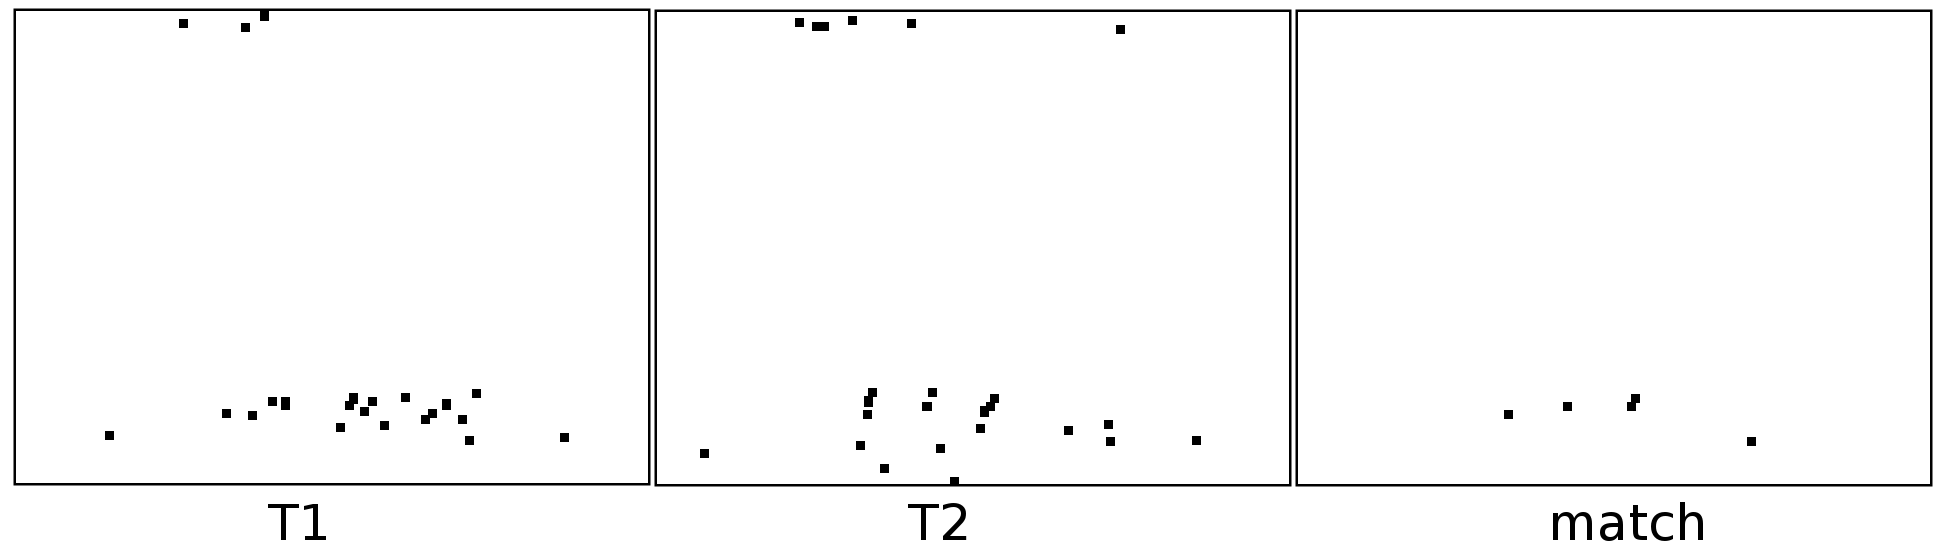
\includegraphics[width=\linewidth]{img/detectedLocations.png}
  \caption{Locations of partially-stuck pixel candidates. Correctly classified pixel defects from $T_1$ are contained in $T_2$ as well. All other detected defects in $T_1$ can be interpreted as misclassification, since they violate the \emph{once defective, always defective}-condition.}
  \label{fig:defectPersistence}
\end{figure}


\begin{eqnarray}
 \lambda_{ps} 	& = 	& \gamma \frac{n_2-n_1}{(T_2-T_1)\cdot(w \cdot h)} \\ 
 \lambda_{s} 	& = 	& \gamma  \frac{n_{s2}-n_{s1}}{(T_2-T_1)\cdot(w \cdot h)} \\
 a_{ps} 	& = 	&max(\hat{D}_{s_k}) \\ 
 a_{s} 		&:= 	& 255
\end{eqnarray}

% TODO: Debiasi14a fehlt...

%%%%%%%%%%%%%%%%%%%%%%%%%%%%%%%%%%%%%%%%%%%%%%%%%%%%%%%%%%%%%%%%%%%%%%%%%%%%%%%%%%%%%%%%%%%%%%%%%%%%%%%%%%%
\section{Experimental setup}
 \label{testing}
 With the proposed method simulation parameters are estimated from a dataset. The dataset used in this work contains iris texture images acquired with the \emph{Irisguard H100 IRT} sensor. The images are divided into 2 data sets, the first one containing images from 49 distinct subjects acquired in 2009 (480 - 1561 images per subject), the second one containing images from exactly the same subjects acquired in 2013 (40 images per subject), resulting in a time gap of four years between the acquisition of the two image sets. These data sets are subsequently denoted as \emph{H100-2009} and \emph{H100-2013}. \emph{H100-2009} is a subset of the CASIA cross sensor iris database \cite{Xiao13a}.

To be able to reliably estimate the sensor defect's growth rate and amplitudes for the mentioned data sets it is essential to ensure that the image sets in 2009 and 2013 have been acquired using an identical iris sensor device. Tthis is of particular interest since doubts on this issue emerged in the context of the CASIA V.4 datasets recently \cite{Debiasi14a}. 
%Therefore we needed to verify that the \emph{Irispass-2009} and \emph{Irispass-2013} data sets have been acquired with the exactly same iris sensor device, as well as the \emph{H100-2009} and \emph{H100-2013} data sets. 
%For this purpose we employ digital image forensic \cite{farid-spm-09} techniques. Sensor fingerprints, a methodology classically used in digital image forensics, are based on a sensor’s photo response non uniformity (PRNU) \cite{12696519,journals/tifs/ChenFGL08} and can be used to prove sample data authenticity by identifying the source sensor uniquely. Even various sensors from the same make/brand and model can be distinguished.
To prove that the sensor device used in 2013 is the same specific device as used in 2009 and vice versa, we adopted the sensor identification methodology of H\"oller and Uhl \cite{UhlH12}. 
We assume that the images under investigation, namely the 2009 and 2013 data sets, are acquired with different sensor devices and derive from the results that this assumption is not correct (proof by contradiction).

We extract the PRNU noise residual of every image from 4 patches located in the corners of the image with a size of 128x128 pixels each. Then from each data set, 2009 and 2013, 850 images are randomly chosen, resulting in a total of 1700 images. From the 850 images per set 50 are used to generate the PRNU fingerprint $\hat{K}$ for the data sets and the other 800 are used to calculate the normalized cross correlation (NCC) scores between fingerprints and noise residuals. 
% At this, the presence of the PRNU fingerprint $\hat{K}$  in the images is examined to obtain the NCC scores.
This leads to 800 matching (fingerprint $\hat{K}$ comes from the same sensor as the images in the data set under investigation) and 800 non-matching NCC scores (fingerprint $\hat{K}$ comes from an other sensor as the images in the data set under investigation) for each sensor.
We then calculate the equal error rate EER from all correlation values $\rho$ by comparing the two data sets. To estimate the real variability of these values, the interval of confidence (CI) at 95\% is estimated. To do so, the calculation of EER and threshold is repeated 1000 times on the respective set of $m$ matching and $n$ non-matching $\rho$ values, by drawing $m$ correlation values from the matching-data set and $n$ correlation values from the non-matching data set, making use of sampling with replacement. As a result, we obtain 1000 EERs and the range containing 95\% of these values is the interval of confidence. 

  \begin{table}[hbt] 
   \begin{center}
	\begin{tabular}{ c | c | c}
		  \emph{Irisguard H100 IRT} & EER & CI \\ 
		  \hline
		   [\%] &  48.93 & $[47.81 , 50.20]$
	\end{tabular}
   \end{center}
     \caption{EER and confidence interval CI for \emph{Irisguard H100 IRT}.}
\label{table:sensor_identification}
 \end{table}

As the results of this experiment in table \ref{table:sensor_identification} indicate, the EER is very high. This means the matching and non-matching NCC scores are almost identical, therefore resulting in an EER of approximately 50\%. Thus the assumed non-matching scores cannot be distinguished from the matching scores, because the the PRNU fingerprints generated from both data sets are present in the images from the same data set as well as in the other data set. This contradicts the assumption that the sensor used in 2009 is different from the sensor used in 2013, hence the same sensor was used to acquire both data sets.

%beweis beide sensoren gleich:
%	- methode fridrich
%	- FP berechnet aus 50 bildern, zufällig
%	- 800 matches und 800 non matches
%	- bilder für FP nicht für matching verwendet
%	- annahme: sensor ist nicht gleich
%	- eer sehr hoch, weil corr scores annähernd gleich für beide datensets
%	- deswegen anahme falsch und es handelt sich um gleichen sensor
%	- konfidenzintervalle
%

Furthermore the PRNU fingerprints of both sensors have been analyzed to provide evidence for eventual sensor ageing. For this purpose, we generate 16 PRNU fingerprints  by extracting the PRNU using a 3x3 median filter for computing noise residuals as proposed by Fridrich \cite{fridrich}, because sensor defects are spiky in nature and a non-linear filter is more likely to extract these defects correctly. The PRNU fingerprints are generated from 50 distinct and randomly chosen images from the 2009 and 2013 data sets (no image has been used in the generation of more than one PRNU fingerprint). 
These fingerprints are used to calculate a couple of pairwise NCC scores among the fingerprints: 2009 intra-set correlations (fingerprints from 2009 with fingerprints from 2009), 2013 intra-set correlations (fingerprints from 2013 with fingerprints from 2013) and 2009-2013 inter-set correlations (fingerprints from 2009 with fingerprints from 2013). Thus we obtain $16^{2}-16 = 240$ NCC scores for each intra-set correlation and $16^2 = 256$ NCC scores for the inter-set correlation. The NCC scores are then averaged by calculating the mean of the scores.
The results in table \ref{table:prnu_fp_corr} show that the NCC scores for fingerprints generated from images of the same time period are clearly higher then NCC scores of the fingerprints over the four year time span. Therefore an alteration of the PRNU fingerprint can be observed over the four year time span, conditioned by the ageing of the sensors.
 
 \begin{table} [hbt]
 \begin{center}
	\begin{tabular}{ c | c | c | c }
		   Period & 2009 - 2009 & 2013 - 2013 & 2009 - 2013 \\
		  \hline
			Mean NCC & 0.1175 & 0.1207  & 0.0911 
	\end{tabular}
	\vspace{2mm}
        \caption{\emph{Irisguard H100 IRT} mean NCC scores showing impact of sensor ageing on PRNU fingerprints generated from images of different time periods.}
    \label{table:prnu_fp_corr}
\end{center} 
\end{table}

\vspace{-4mm}

Since we proved the images were indeed acquired using the same sensor and show ageing effects, we use the method described in section \ref{hotPixelRate} to retrieve growth rate and amplitudes of pixel defects for the \emph{Irisguard H100 IRT}. Lacking the sensor's setting information for images in the data set, we have to assume no in-field defect correctiond \cite{inFieldDefects} were mad and exposure settings were constant for all acquisition processes. By chosing a 9x9 median kernel and appropriate $\tau_{ps}$ as decision thresholds, $n_{ps}=27$ and $n_{ps}=28$ candidates for partially-stuck pixels were found in 2009 and 2013 respectively (see fig. \ref{fig:defectPersistence}). Because there where $n_{match}=5$ matching pixels, the correction factor is set to $\gamma=0.185$. Using these values, an estimated growth rate $\lambda_{ps}=0.66594$ can be determined. The growth rates are measured in \emph{number of defects per Megapixel per year}. The retrieved values (refer table \ref{table:parameters}) correspond well with the findings of others \cite{defectDetection, leung}. Dudas suggests in \cite{inFieldDefects} that real stuck pixels are never detected in field, because they are easy to detect at fabrication time and get corrected or may correspond to partially stuck pixels with extremely high offset. However, we modelled actual stuck pixels at a moderate growth rate (refer table \ref{table:tests}) to investigate what happens if stuck pixels should occur. Furthermore, we modelled other sensors with growth rates retrieved from literature and pushed the ageing parameters to mutiples of the real values. A summary of all used parameters in this simulation is given in table \ref{table:parameters}.

 % TODO: Proof of correctness by probability

 \bgroup
\def\arraystretch{1.3}%  1 is the default, change whatever you need
 \begin{table} [hbt]
  \begin{center}
    \begin{tabular}{|c | c c c|}
    \hline 
    \textbf{Parameters} & h100  & APS \cite{leung} & CCD \cite{leung} \\
    \hline 
    $\lambda_{ps} [\frac{\text{defects}}{\text{year} \cdot 10^6 \text{pixels}}]$  & 0.6659 &  0.7432 & 0.5694 \\
    $\lambda_s$ 	&  0  & 0 & 0 \\
    $a_s$		&  255  & 255 & 255 \\
    $a_{ps}$	&  3  & ? & ? \\
    \hline  
    \end{tabular}

    \vspace{1mm}
    \hfill \tiny { $1MP := 10^6 pixels$}
     \vspace{-2mm}
    
    \caption{Simulation parameters. }
    \label{table:parameters}
  \end{center}
  \vspace{-5mm}
\end{table}

\egroup

 Based on these parameters, a number of virtual sensors are defined in table \ref{table:tests}, where sensor A corresponds to the \emph{Irisguard H100 IRT}. They are designed in a way that all possible combinations of stuck and partially-stuck pixels are covered. Sensors F,G and H show amplitudes and growth rates which are very unlikely to be observed in practice, but should demonstrate the impact of strong ageing effects. 
 
 \begin{table}[bt]  
  \begin{center}
  \begin{tabular}{c | c c c }
  Sensor & $\lambda_{ps}$ & $\lambda_{s}$ & $a_{ps}$  \\
  \hline
  A	&	$\lambda_{h100}$ & 0 & $a_{ps_{h100}}$ \\
  B & $\lambda_{h100}$ & $\lambda_{APS}$ & $a_{ps_{h100}}$ \\
  C & $\lambda_{APS}$ & 0 & $a_{ps_{h100}}$    \\
  D & $\lambda_{CCD}$ & 0 & $a_{ps_{h100}}$   \\
  E & 0 & $\lambda_{APS}$ & -- \\
  F & $ 4 \lambda_{h100}$ & 0 & $ 2 a_{ps_{h100}}$ \\
  G & $ 4 \lambda_{h100}$ & 0 & 100 \\
  H & $ 8 \lambda_{h100}$ &  $ 5 \lambda_{APS}$ & 100

  \end{tabular}
    
    \vspace{3mm}
    \caption{Virtual sensors for simulation}
    \label{table:tests}
  \end{center}
 \end{table}
  
  Six implementations 
  %\cite{Ma,Monro,ko,rathgeb} 
  of iris-signature algorithms provided by the USIT Framework v1.0.3 (as available at \url{http://wavelab.at/sources/} \cite{rathgeb}) are tested for vulnerability to sensor ageing. In the semgentation step, weighted adaptive Hough and ellipsopolar transform (WAHET \cite{wahet}) is used. For each of the virtual sensor models in table \ref{table:tests}, an aged data set based on the IITD iris database v1.0 (TIFF, N=2240) \cite{IITD} over a time span of 96 years (8 year steps) is calculated. The impact of sensor ageing is determined by evaluation of the Equal Error Rate (EER). In terms of this paper the EER is calculated by considering the left and right eye as seperate classes. By the structure of the database, 8940 genuine and 5006400 impostor matches are used for computing the EER with crossover evaluation.
  
 \section{Results}
 \label{results}
 Two algorithms of Rathgeb and Uhl (abbreviated \emph{cb} and \emph{cr}) 
 %\cite{rathgeb}
 and the algorithms of Ko \etal,
 %\cite{ko}
Monro \etal (\emph{dct}),
 %\cite{Monro}
 Ma \etal(\emph{qsw})
 %\cite{Ma}
  and the LogGabor-1D method by L. Masek (\emph{lg}) as (re-)implemented in USIT were tested with aged data sets generated with the sensor models proposed in table \ref{table:tests}.
 
 Figure \ref{fig:sensor1} shows the developments of the EER as sensor A ages. For none of the six tested algorithms a trend in the progress of the EER can be observed. This means, the effects of sensor ageing do not decrease an iris recognition system's accuracy in general. There is, however, a significant variation in the EER for some of the algorithms. The methods \emph{cb} and \emph{ko} are robust against defects caused by sensor ageing. While three of the other algorithms are considered to be widely stable, the LogGabor-1D is sensitive to ageing-related defects. 
 
  \begin{figure}
  \centering
  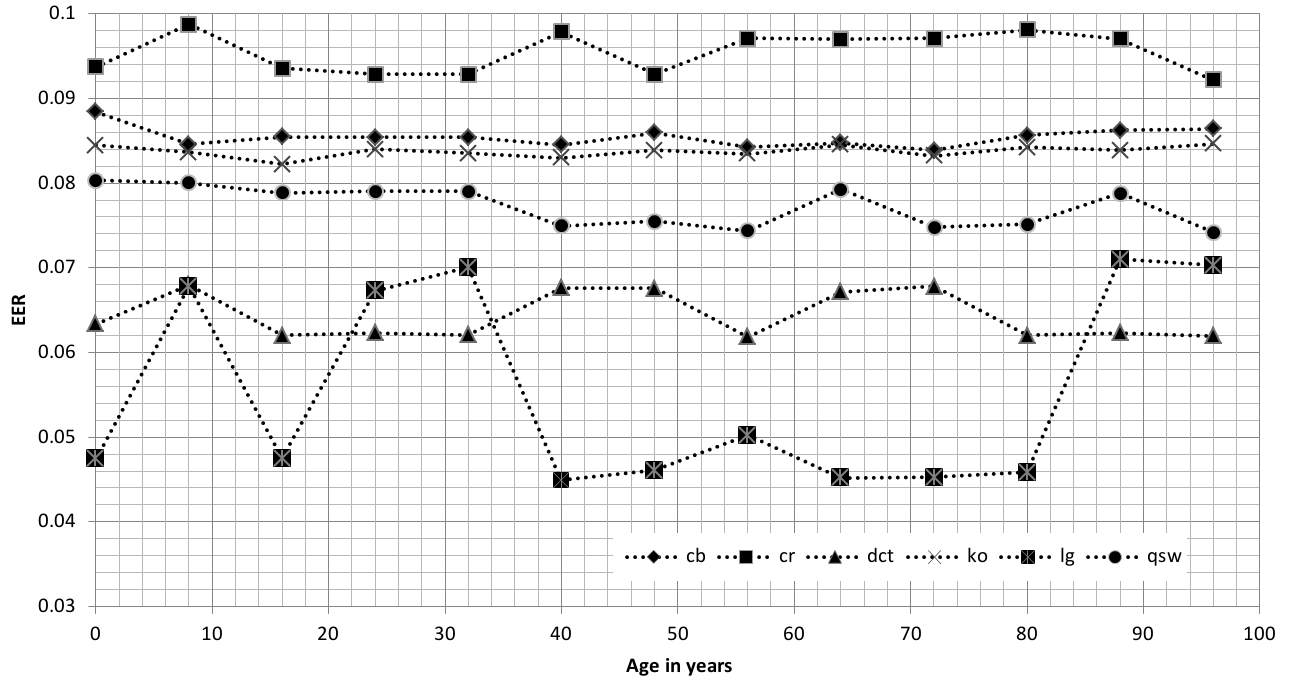
\includegraphics[width=\linewidth]{img/sensor1.png}
  \caption{EER of six iris-signature algorithms using Sensor A. Note that EERs are high, because of the used WAHET-segmentation. Other segmentation methods might result in generally lower EER rates.}
  \label{fig:sensor1}
\end{figure}

This means that some algorithms, i.e. LogGabor-1D in this case, showing high EER variance are not robust towards spiky noise in the sensor output, which is often caused by ageing defects. This noise influences both stages of an iris recognition system, namely the segmentation and/or the generation of the iris code / template. Since the impact on the segmentation step has not been explicitely investigated, it cannot be distinguished whether one of the tested iris-feature extraction algorithms is sensitive to spiky noise in the segmented image, commonly denoted as iris texture, or to changes in the segmentation behaviour itself. Since the same segmentation was used for all tests, it is indeed possible to see from the results that systems using robust algorithms, such as \emph{cb} or \emph{ko}, tend to be more robust towards spiky noise caused by ageing-related defects than others. This holds as long as systems with the same segmentation methods are used.
 
  \begin{figure}
  \centering
  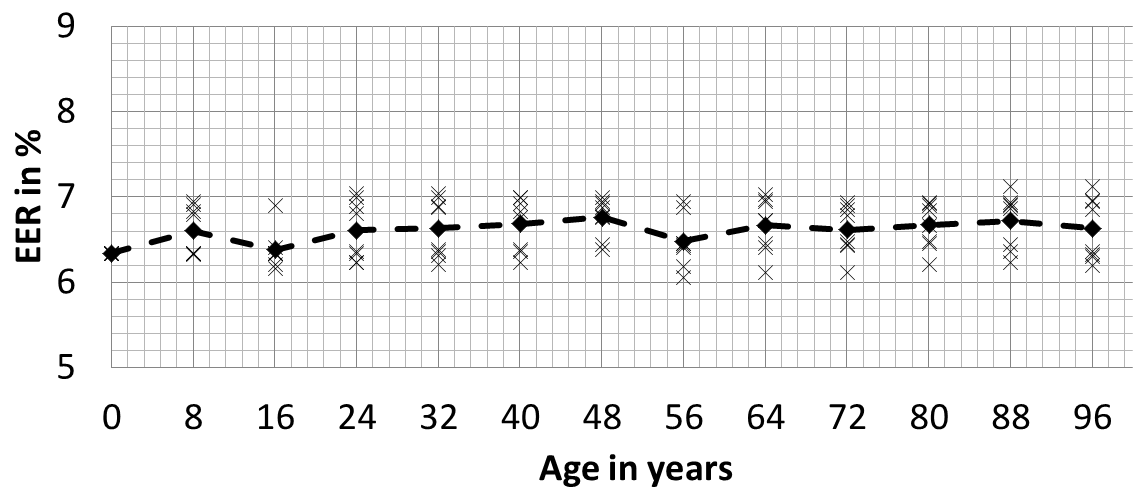
\includegraphics[width=\linewidth]{img/dct.png}
  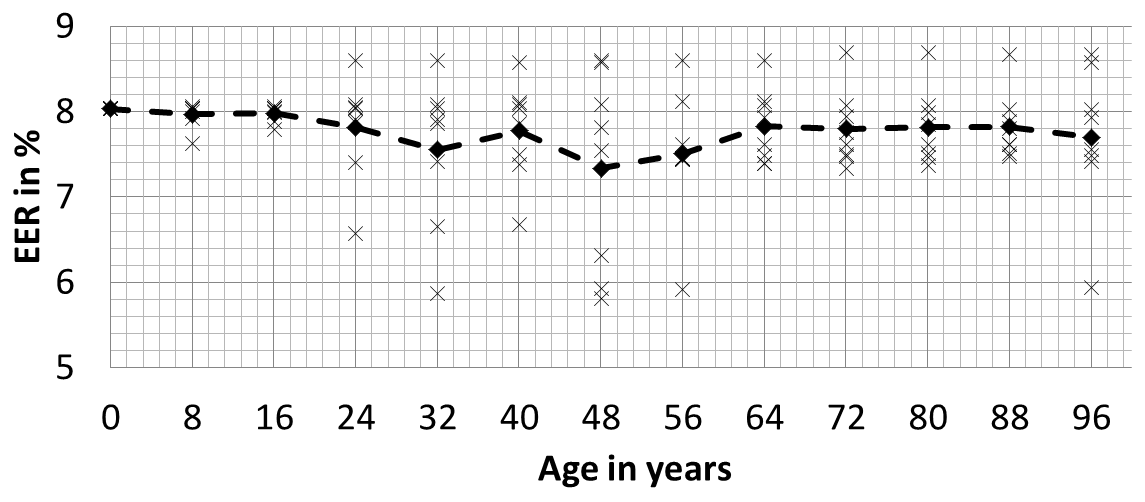
\includegraphics[width=\linewidth]{img/qsw.png}
  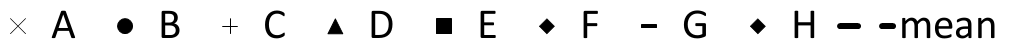
\includegraphics[width=\linewidth]{img/legend.png}
  %\caption{Equal error rates of the algorithms of Monro \etal (top) and Ma \etal \cite{Ma} (bottom). EER for data sets corresponding to sensors A-H at sample times are plotted as unlabelled data points. The mean EER over all data sets is plotted as dashed line.}
  \caption{Equal error rates of the algorithms of Monro \etal (top) and Ma \etal (bottom) for aged data sets corresponding to sensors A-H. The mean EER over all data sets is plotted as dashed line.}
  \label{fig:allSensors}
\end{figure}
 
 When the same iris feature extraction algorithm is used with data sets created using the virtual sensor models A-H, one can investigate the general robustness of a specific algorithm. This is the case, because sensors with different ageing characteristics (growth rate, amplitude, defect-types) are taken into account in this experiment. Figure \ref{fig:allSensors} illustrates the average EER for the algorithms of Monro \etal and Ma \etal over data sets generated from all sensor models. For each sample point in time, EER-points corresponding to the sensor models are plotted. This visualizes the variance of the EER between data sets, hence the impact of distribution and strength of ageing related defects. The algorithms of Monro \etal (\emph{dct}) and Ma \etal (\emph{qsw}) were chosen as an illustrative example, because a similar variance is indicated by their graphs in figure \ref{fig:sensor1}. The distribution of EER-samples in the plot in figure \ref{fig:allSensors} reveals that the algorithm of Monro \etal shows much lower variance in general than the one of Ma \etal. This contradicts the initial observation from \ref{fig:sensor1}, which means it is crucial to run multiple simulations with different sensor models to give a statement on the general robustness towards sensor ageing. Interestingly, Sensor E, which has stuck pixels only, tends have the highest impact, whereas this would have been expected for sensor H, which has the strongest aging characteristics. However, both sensor models have pushed growth rates and amplitudes. For sensors A-C, which are realistic models, no such trend is observable.
 
 \section{Conclusion}
 \label{conclusion}
% We used a simulation to add ageing-related defects to a data set of already acquired sensors outputs, namely images. Practical relevance has been established by retrieving simulation parameters from data, which has been captured by an iris scanner in a 4 years' difference. To retrieve these parameters, a method was proposed in section \ref{hotPixelRate}. Using them and similar ones from related work, an experiment has been carried out, as discussed in section \ref{testing}. From the results we conclude on the impact of sensor-ageing on iris recognition systems.
 
The results indicate that iris recognition systems are influenced by sensor aging. Although for practical applications, no general decrease in the recognition rate was observed, there is, however, a potentially significant sensitiveness towards spiky noise, i.e. caused by sensor ageing. This means an iris recognition system's accuracy depends on the current physical condition of the sensor - which changes over time. We showed that defects related to sensor ageing influence the accuracy of an iris recognition system in a transitory way. The results of experiments aiming to investigate iris texture ageing, which were obtained by evaluation of the change in a system's accuracy (e.g. the EER), can not be considered entirely reliable for this reason, since the different physical states of the sensor at data acquisition might have significant impact on the results.  
 
 % TODO: Claim that this might void the results of all that claim that a decrease in detection accuracy is true when a human ages ==> Sensor might be in a transitory bad state.
 

 %\section{Future work}
 %\begin{itemize}
 % \item Detect hot/stuck pixels by laboratory measurements. Compare to the observed method
 % \item Also no true stuck pixel http://euler.ecs.umass.edu/research/ctkk-spie-2013.pdf
 %\end{itemize}


% ------------------------ Reference section

{\small
\bibliographystyle{ieee}
\bibliography{ijcb}
}

% TODO: Table referencing does not work!!
% TODO: Figure 2 enhance

\end{document}
